\documentclass[xcolor=pdftex,svgnames,table]{beamer}
\usepackage{latexsym,amssymb,amsmath,stmaryrd}
\usepackage[utf8]{inputenc}
\usepackage[T1]{fontenc}
\usepackage[francais]{babel}
\usepackage{pgf}
\usepackage{tikz}
\usetikzlibrary{arrows,patterns,plotmarks,shapes,snakes,er,3d,automata,%
backgrounds,topaths,trees,petri,mindmap}
\usepackage{pgfbaseimage}
\usepackage{ifpdf}
\ifpdf
\usepackage{graphicx}
\else
%\usepackage[dvips]{graphicx}
\usepackage{pstricks,pst-tree,pst-node}
\newpsobject{showgrid}{psgrid}{subgriddiv=1,griddots=10,gridlabels=6pt}
\fi
\usepackage{moreverb}
\usepackage[normalem]{ulem}
\usepackage{version}
\usepackage{url}
\usepackage{multicol}
\usepackage{listings}
\lstset{
  language=[ANSI]C, 
%  gobble=2, 
%  escapeinside="", 
  basicstyle=\ttfamily, 
%  directivestyle=\color{Fuchsia},
  identifierstyle = \color{DarkOrange},
  keywordstyle=\color{DarkGreen}, 
  commentstyle=\color{red}, 
%  numbers=left, 
%  numbersep=5pt, 
%  numberstyle=\scriptsize, 
%  moredelim=[is][\color{gray}\itshape]{/*}{*/}, 
%  moredelim=[is][\alert]{/+}{+/}, 
%  morecomment=[is]{/=}{=/}, 
%  morecomment=[in]{comment=}{,} 
%  fancyvrb=true 
} 

\newcommand{\binaire}[1]{\ensuremath{\underline{#1}}}
\newcommand{\C}[1]{\texttt{#1}}
\newcommand{\bbbn}{\ensuremath{\mathbb{N}}}
%%%%%%%%%%%%%%%%%%%%%%%%%%%%%%%%%%%%%%%%%%%%%%%%%%%%%%%%%%%%%%%%
%% ccBeamer 0.1, 2007-07-02                                   %%
%% Written by Sebastian Pipping <webmaster@hartwork.org>      %%
%% ---------------------------------------------------------- %%
%% Licensed under Creative Commons Attribution-ShareAlike 3.0 %%
%% http://creativecommons.org/licenses/by-sa/3.0/             %%
%%%%%%%%%%%%%%%%%%%%%%%%%%%%%%%%%%%%%%%%%%%%%%%%%%%%%%%%%%%%%%%%


%% Images
\newcommand{\CcImageBy}[1]{%
	
\includegraphics[scale=#1]{creative_commons/cc_by_30}%
}
\newcommand{\CcImageCc}[1]{%
	
\includegraphics[scale=#1]{creative_commons/cc_cc_30}%
}
\newcommand{\CcImageDevNations}[1]{%
	
\includegraphics[scale=#1]{creative_commons/cc_dev_nations_30}%
}
\newcommand{\CcImageNc}[1]{%
	
\includegraphics[scale=#1]{creative_commons/cc_nc_30}%
}
\newcommand{\CcImageNd}[1]{%
	
\includegraphics[scale=#1]{creative_commons/cc_nd_30}%
}
\newcommand{\CcImagePd}[1]{%
	
\includegraphics[scale=#1]{creative_commons/cc_pd_30}%
}
\newcommand{\CcImageSa}[1]{%
	
\includegraphics[scale=#1]{creative_commons/cc_sa_30}%
}
\newcommand{\CcImageSampling}[1]{%
	
\includegraphics[scale=#1]{creative_commons/cc_sampling_30}%
}
\newcommand{\CcImageSamplingPlus}[1]{%
	
\includegraphics[scale=#1]{creative_commons/cc_sampling_plus_30}%
}


%% Groups
\newcommand{\CcGroupBy}[1]{% zoom
	\CcImageBy{#1}%
}
\newcommand{\CcGroupByNc}[2]{% zoom, gap
	\CcImageBy{#1}\hspace*{#2}\CcImageNc{#1}%
}
\newcommand{\CcGroupByNcNd}[2]{% zoom, gap
	\CcImageBy{#1}\hspace*{#2}\CcImageNc{#1}\hspace*{#2}\CcImageNd{#1}%
}
\newcommand{\CcGroupByNcSa}[2]{% zoom, gap
	\CcImageBy{#1}\hspace*{#2}\CcImageNc{#1}\hspace*{#2}\CcImageSa{#1}%
}
\newcommand{\CcGroupByNd}[2]{% zoom, gap
	\CcImageBy{#1}\hspace*{#2}\CcImageNd{#1}%
}
\newcommand{\CcGroupBySa}[2]{% zoom, gap
	\CcImageBy{#1}\hspace*{#2}\CcImageSa{#1}%
}
\newcommand{\CcGroupDevNations}[1]{% zoom
	\CcImageDevNations{#1}%
}
\newcommand{\CcGroupNcSampling}[2]{% zoom, gap
	\CcImageNc{#1}\hspace*{#2}\CcImageSampling{#1}%
}
\newcommand{\CcGroupPd}[1]{% zoom
	\CcImagePd{#1}%
}
\newcommand{\CcGroupSampling}[1]{% zoom
	\CcImageSampling{#1}%
}
\newcommand{\CcGroupSamplingPlus}[1]{% zoom
	\CcImageSamplingPlus{#1}%
}


%% Text
\newcommand{\CcLongnameBy}{Attribution}
\newcommand{\CcLongnameByNc}{Attribution-NonCommercial}
\newcommand{\CcLongnameByNcNd}{Attribution-NoDerivs}
\newcommand{\CcLongnameByNcSa}{Attribution-NonCommercial-ShareAlike}
\newcommand{\CcLongnameByNd}{Attribution-NoDerivs}
\newcommand{\CcLongnameBySa}{Attribution-ShareAlike}

\newcommand{\CcNote}[1]{% longname
	This work is licensed under the \textit{Creative Commons #1 3.0 License}.%
}

\usetheme{classic}
\newcommand{\nowrite}{\put(10,-4){\includegraphics[scale=.05]{creative_commons/nopencil}}}
\newcommand{\youwrite}{\put(10,-4){
\includegraphics[scale=.05]{creative_commons/pencil}}}
\newcommand{\writethat}{
\includegraphics[scale=.05]{creative_commons/pencil}}
\newcommand{\aemporter}{\put(10,-6){
\includegraphics[scale=.05]{creative_commons/szymonraj_Shopping_bag}}}


%%% Titre -- cours 9
\title{Éléments d'informatique -- Cours 9.\\ Fonctions (2)}
\author{Pierre Boudes}
\date{\today}

\begin{document}

%% Page de titre et licence CC.
\begin{frame}
	\titlepage
	\vfill
	\begin{center}
		\CcGroupByNcSa{0.83}{0.95ex}\\[2.5ex]
		{\tiny\CcNote{\CcLongnameByNcSa}}
		\vspace*{-2.5ex}
	\end{center}
\end{frame}

%%%%%%%%%%%%%%%%%%%%
\section[Plan]{}
\frame[label=plan]{\tableofcontents}
\section{Types}
\subsection{Types en C et entrées/sorties associées}

\begin{frame}
  \frametitle{Types en C et entrées/sorties associées}  
Type des caractères \alert{\C{char}} :
    \begin{itemize}
    \item Déclaration et initialisation : \C{char c = 'A';}.
    \item Représentation sur 8 bits, ASCII, ISO-8859-x, UTF-8.
    \item E/S : \alert{\C{\%c}}.
    \end{itemize}

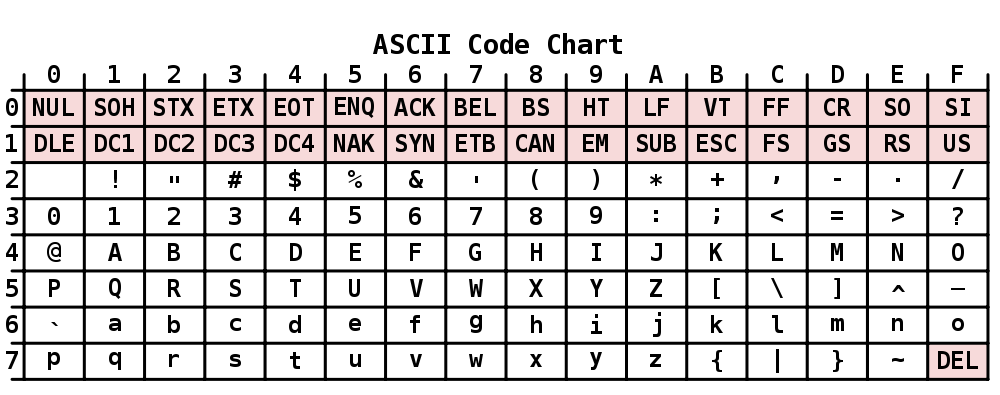
\includegraphics[scale=0.31]{img/1000px-ASCII_Code_Chart.png}

\vspace{-0.3cm}
{\scriptsize\hfill  Source: Wikimedia Commons, public domain.}
\end{frame}

\subsection[Conversions]{Conversions automatiques entre types}
\begin{frame}[fragile]
  \frametitle{Conversions  automatiques entre types}
\pause
  \begin{itemize}
\item Sans changement de représentation  :
  \begin{itemize}
    \item \C{char} vers \C{int}
    \item \C{int} vers \C{char} (troncature)
  \end{itemize}\pause
  \begin{lstlisting}[basicstyle=\ttfamily\small] 
  char c;
  int n;
  
  n = 'A' + 1;
  c = n + 24;
   \end{lstlisting}  \pause
 \item Avec changement de représentation :
    \begin{itemize}
    \item char ou entiers vers réels
    \item réels vers entiers ou char
    \end{itemize}
  \begin{lstlisting}[basicstyle=\ttfamily\small] 
  double x;
  int n;
  
  n = 3.1;
  x = n;
   \end{lstlisting}  \pause
  \end{itemize}
\end{frame}

\section{Pile d'appel}
\subsection{Rappel sur les fonctions en C}
\begin{frame}
  \frametitle{Rappel sur les fonctions en C\nowrite}
 Utilisation des fonctions :
  \begin{itemize}
    \item \structure{déclaration} (types des paramètres et de la valeur de retour)
    \item \structure{définition}  (code, paramètres formels)
    \item \structure{appel} (paramètres effectifs, \textbf{espace mémoire})
  \end{itemize}
\pause
Voyons de manière plus précise cette question d'espace mémoire.
\end{frame}

\subsection{Traces et mémoire}
\begin{frame}
  \frametitle{Traces et mémoire \nowrite}
\noindent \structure{Rappel :} 
nous faisons la trace de chaque appel de chaque fonction que
l'on a défini (pas les fonctions externes, comme printf). 

\pause
\begin{columns}
\column[T]{6cm}
La trace d'un programme donne schématiquement ce type de dessin
\begin{itemize}
  \item<3-> verticalement, c'est le temps
  \item<3-> et horizontalement, l'occupation mémoire
  \item<4-> un appel de fonction occupe une portion de mémoire, puis la
    libère. 
\item<5-> la trace représente réellement ce qui arrive dans vos programmes.
\end{itemize}
 \uncover<6->{
\structure{Un appel de fonction peut-il modifier la mémoire d'une
  fonction appelante ?}}

\column[T]{4.5cm}
\vspace{-.5cm}
\small
\only<2->{\noindent\begin{tikzpicture}
\tikzstyle{every node}=[anchor=base]
\only<3->{\tikzset{axis/.style={fill=none}}}
\only<2>{\tikzset{axis/.style={color=white,fill=white,draw=white}}}
% Axis
  \draw[axis,arrows = ->] (-.7,5.9) -- (4.2,5.9);
  \draw(4.1,6) node[axis,anchor=base east] {mémoire};
  \draw[axis,arrows = ->] (-.6,6.1) -- (-.6,-.5);
  \draw(-.8,-.2) node[axis,rotate=-90,anchor=base east] {temps};
%
 \draw (0, 5.6) node {main()};
  \filldraw[fill=LightGreen,draw=Green] (-0.5,-0.25) rectangle
  (1,5.5); 
  \draw[pattern color=Green, pattern=north east lines,draw=none] (-0.5,-0.25) rectangle
  (0,5.5); 
 \draw (0.25, 5.25) node {\C{x}};
  \draw[draw=Green] (0.5,-0.25) -- (0.5,5.5);
  \draw (0.75, 5.25) node {\C{y}};
%
 \draw (1.75, 5.1) node {max(1,2)};
  \filldraw[fill=LightGoldenrod, draw=DarkGoldenrod] (1,4) rectangle (2.5,5); 
  \draw[pattern color=DarkGoldenrod, pattern=north east lines,draw=none] (1,4) rectangle
  (1.5,5); 
  \draw (2.25, 4.75) node {\C{b}};
  \draw[draw=DarkGoldenrod] (2,4) -- (2,5); 
  \draw (1.75, 4.75) node {\C{a}};
%
  \draw (1.75, 3.6) node {\C{f(8)}};
  \filldraw[fill=PowderBlue,draw=RoyalBlue]
  (1,0) rectangle (2.5,3.5); 
  \draw[pattern color=RoyalBlue, pattern=north east lines,draw=none]
  (1,0) rectangle  (1.5,3.5); 
  \draw (1.75, 3.25) node {\C{z}};
  \draw[draw=RoyalBlue] (2,0) -- (2,3.5); 
  \draw (2.25, 3.25) node {\C{r}};
%
  \draw (3, 3.1) node {\C{g(2)}};
  \filldraw[fill=Salmon,draw=Crimson] (2.5,2) rectangle(3.5,3); 
  \draw[pattern color=Crimson, pattern=north east lines,draw=none]
  (2.5,2) rectangle  (3,3);
  \draw (3.25, 2.75) node {\C{n}};
%
  \filldraw[fill=LightGoldenrod, draw=DarkGoldenrod] (2.5,.5) rectangle
  (4,1.5); 
  \draw[pattern color=DarkGoldenrod, pattern=north east lines,draw=none] (2.5,.5) rectangle
  (3,1.5); 
  \draw (3.25, 1.6) node {max(2,-1)};
  \draw (3.25, 1.25) node {\C{a}};
  \draw[draw=DarkGoldenrod] (3.5,.5) -- (3.5,1.5);
  \draw (3.75, 1.25) node {\C{b}};
\end{tikzpicture}}
  \end{columns}
\end{frame}

\subsection{Pile d'appel}
\begin{frame}
  \frametitle{Pile d'appel}
\begin{columns}
\column[T]{4cm}
On parle de \alert{pile d'appel} car les appels de fonctions
s'empilent... \emph{comme sur une pile
    d'assiettes.}

\uncover<13->{
\structure{Peut-on avoir deux assiettes identiques dans la pile ? (La même
  fonction avec des contenus différents)}}

% de contenus différents
\column[T]{7.5cm}
\small
\noindent\begin{tikzpicture}[rotate=90]
\tikzstyle{every node}=[anchor=base]
\tikzset{axis/.style={fill=none}}
\tikzset{fonction/.style={rotate=90}}
% Axis
  \draw[axis,arrows = ->] (-.7,5.9) -- (4.2,5.9);
  \draw(4.1,6) node[axis,rotate=90,anchor=base east] {mémoire};
  \draw[axis,arrows = ->] (-.6,6.1) -- (-.6,-.5);
  \draw(-.8,-.2) node[axis,anchor=base east] {temps};
%
\uncover<1,3->{
  \draw (0, 5.6) node[fonction] {main()};
  \filldraw[fill=LightGreen,draw=Green] (-0.5,-0.25) rectangle
  (1,5.5); 
  \draw[pattern color=Green, pattern=north east lines,draw=none] (-0.5,-0.25) rectangle
  (0,5.5); 
 \draw (0.25, 5.25) node {\C{x}};
  \draw[draw=Green] (0.5,-0.25) -- (0.5,5.5);
  \draw (0.75, 5.25) node {\C{y}};
}
%
\uncover<1,4,12->{
 \draw (1.75, 5.1) node[fonction] {max(1,2)};
  \filldraw[fill=LightGoldenrod, draw=DarkGoldenrod] (1,4) rectangle (2.5,5); 
  \draw[pattern color=DarkGoldenrod, pattern=north east lines,draw=none] (1,4) rectangle
  (1.5,5); 
  \draw (2.25, 4.75) node {\C{b}};
  \draw[draw=DarkGoldenrod] (2,4) -- (2,5); 
  \draw (1.75, 4.75) node {\C{a}};
}
%
\uncover<1,6-10,12->{
  \draw (1.75, 3.6) node[fonction] {\C{f(8)}};
  \filldraw[fill=PowderBlue,draw=RoyalBlue]
  (1,0) rectangle (2.5,3.5); 
  \draw[pattern color=RoyalBlue, pattern=north east lines,draw=none]
  (1,0) rectangle  (1.5,3.5); 
  \draw (1.75, 3.25) node {\C{z}};
  \draw[draw=RoyalBlue] (2,0) -- (2,3.5); 
  \draw (2.25, 3.25) node {\C{r}};
}
%
\uncover<1,7,12->{
  \draw (3, 3.1) node[fonction] {\C{g(2)}};
  \filldraw[fill=Salmon,draw=Crimson] (2.5,2) rectangle(3.5,3); 
  \draw[pattern color=Crimson, pattern=north east lines,draw=none]
  (2.5,2) rectangle  (3,3);
  \draw (3.25, 2.75) node {\C{n}};
}
%
\uncover<1,9,12->{
  \filldraw[fill=LightGoldenrod, draw=DarkGoldenrod] (2.5,.5) rectangle
  (4,1.5); 
  \draw[pattern color=DarkGoldenrod, pattern=north east lines,draw=none] (2.5,.5) rectangle
  (3,1.5); 
  \draw (3.25, 1.6) node[fonction] {max(2,-1)};
  \draw (3.25, 1.25) node {\C{a}};
  \draw[draw=DarkGoldenrod] (3.5,.5) -- (3.5,1.5);
  \draw (3.75, 1.25) node {\C{b}};
}
\end{tikzpicture}
\end{columns}
\end{frame}

\begin{frame}[fragile]
  \frametitle{Factorielle récursive (teaser)}
  \begin{block}{Définition}
    Une fonction récursive est une fonction dont la définition fait
    appel à la fonction \emph{elle-même}.
  \end{block}

\pause
Il y a une forte analogie avec les maths : $(n + 1)! = (n + 1) \times n!$

\pause
\begin{lstlisting}[escapechar={\%},basicstyle=\ttfamily\small] 
int factorielle(int n)
{
    if (n < 2) /* cas de base */
    {
         return 1;
    } 
    return n * factorielle(n - 1); 
}
\end{lstlisting}
\end{frame}

\section[math.h]{Utiliser les
  fonctions d'une bibliothèque}

\begin{frame}[fragile]
  \frametitle{Utiliser les fonctions d'une bibliothèque (math.h)}
Utilisation de la bibliothèque math.h 
\begin{verbatim}
$ man math
\end{verbatim}
  \begin{block}{Déclarer}
    \begin{lstlisting}[basicstyle=\ttfamily\small] 
#include <math.h>
     \end{lstlisting}
  \end{block}

  \begin{block}{Appeler}
  \begin{lstlisting}[basicstyle=\ttfamily\small] 
  double x;

  x = log(3.5);
    \end{lstlisting}  
  \end{block}

  \begin{block}{Définir}
\begin{verbatim}
$ gcc -lm -Wall prog.c -o prog.exe
\end{verbatim}
 \end{block}
\end{frame}


\section[Démos]{Longue démo (menu)}
\begin{frame}
  \frametitle{Longue démo (menu)}
\end{frame}
\end{document}

% revenir sur :
%-l'appel au cours suivant : paramètre et expression, pile d'appel.
%-la grammaire des identificateurs